\documentclass[10pt,letterpaper]{article} 
%\usepackage{tikz}
%\usepackage{tools}
\usepackage{amsmath,amssymb,geometry,graphicx,enumitem}
%\usefonttheme{serif}‎
%\usepackage{ptext}‎
\usepackage{xepersian}
%\settextfont{B Nazanin}
%\usepackage{lipsum}
\setlength{\parindent}{0mm}
\setlength{\parskip}{3mm}
%\newcommand{\pf}{$\blacksquare$}
\newcounter{questionnumber}
\setcounter{questionnumber}{1}
\newcommand{\Q}{
\textbf{سوال \thequestionnumber)}
\stepcounter{questionnumber}
}
\newcommand{\eqn}[1]{
\[
\begin{split}
#1
\end{split}
\]
}
%\newcommand{\EX}{\Bbb E}
%\newcommand{\nl}{\newline\newline}


\begin{document}
\newgeometry{top=15mm,right=15mm,left=15mm,bottom=15mm}

\large
\begin{center}
به نام زیبایی

\begin{table}[h]
\centering
\begin{tabular}{rr}
پایان ترم شبکه‌های مخابرات نوری
\hspace{50mm}
&
زمان: 2 ساعت
\\
نام و نام خانوادگی:
&
شماره‌ی دانشجویی:
\end{tabular}
\end{table}

\hrulefill
\end{center}

\Q
در شبکه‌ی 4 نوده‌ی زیر، تقویت کننده ها با مثلث و فیبرها به صورت سیم پیچ نشان داده شده اند. لینک ها یک طرفه هستند.
\begin{figure}[ht]
\centering
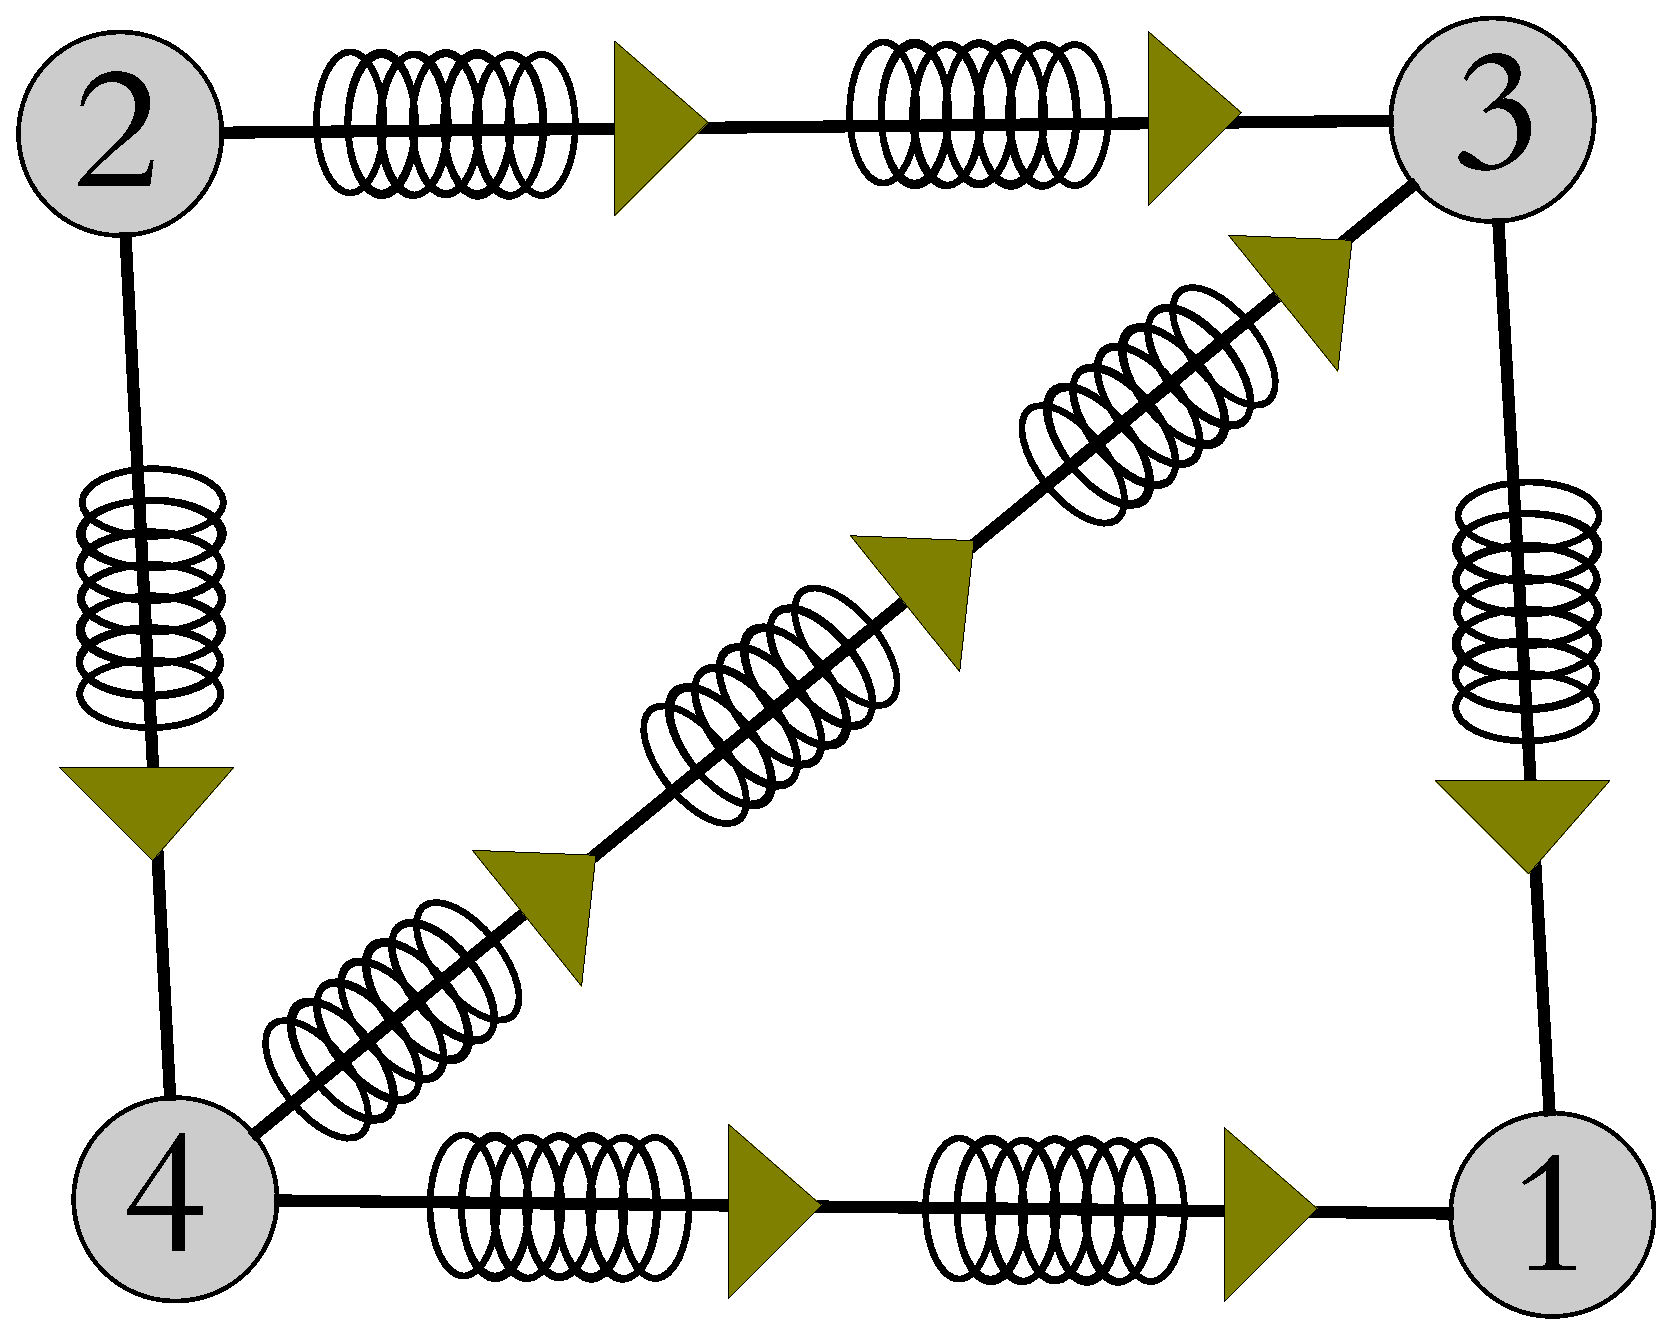
\includegraphics[scale=0.2]{PS1_Net}
\end{figure}

الف) این شبکه چند لینک و اسپن دارد؟

ب) با فرض اینکه هر نود روی هر درجه‌ی ورودی خود، دارای یک تقویت کننده به نام پیش‌تقویت‌کننده وروی هر درجه خروجی خود دارای یک تقویت کننده به نام بوستر است، دو نود را که به ترتیب دارای بیشترین تعداد پیش‌تقویت‌کننده و بیشترین تعداد بوستر هستند نام ببرید.

\hrulefill

\Q

ساختار سوئیچینگ نوری زیر را در نظر بگیرید که یک اسپلیتر (جداساز) دارای $N$ درگاه خروجی وجود دارد و در هر یک از درگاه‌های آن، یک WSS با یک ورودی و $N$ خروجی نصب شده است.
\begin{figure}[h]
\centering
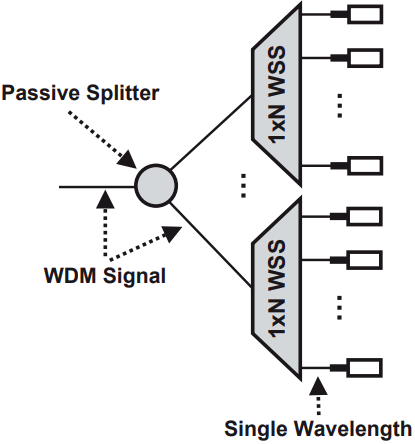
\includegraphics[scale=0.5]{Q2.png}
\end{figure}

اکنون، ساختار دیگری را در نظر بگیرید دارای یک WSS با یک ورودی و $N$ خروجی  است و در هر یک از پایانه‌های آن، یک اسپلیتر نصب شده است. این دو ساختار را از منظر هزینه، توان سیگنال و قابلیت مالتی‌کست با یکدیگر مقایسه کنید.

\hrulefill

\Q
یک سیستم انتقال نوری، شامل یک فیبر نوری به همراه دو طبقه تقویت کننده است. در طبقه‌ی اول، تقویت کننده‌ی رامان با حداکثر بهره‌ی 20dB و در طبقه‌ی دوم، تقویت کننده‌ی EDFA با حداکثر بهره‌ی 7dB است. طول فیبر، 80 کیلومتر و ضریب تضعیف آن، 
$
0.2\text{dB/km}
$
است. تقویت‌کننده‌ی EDFA دارای عدد نویز ثابت 5dB و تقویت‌کننده‌ی رامان، به ازای بهره‌ی تقویت کننده‌ی 13dB ، برابر 21dB است و با هر 1dB افزایش در بهره‌ی تقویت‌کننده‌ی رامان، dB$0.25$ افت می‌کند. بهره‎‌ی هر دو تقویت‌کننده را به گونه‌ای بیابید که بهره‌ی سیستم انتقال (تلفات فیبر به همراه بهره‌ی تقویت‌کننده‌ها) برابر 0dB شود و عدد نویز این سیستم، کمترین مقدار ممکن باشد. سپس این مقدار را بیابید.

(راهنمایی: در یک سیستم با دو طبقه تقویت‌کننده که بهره‌ی خطی و عدد نویز خطی تقویت‌کننده‌ی طبقه اول برابر
$
G_1
$
و
$
F_1
$
و بهره‌ی خطی و عدد نویز خطی تقویت‌کننده‌ی طبقه دوم برابر
$
G_2
$
و
$
F_2
$
است، عدد نویز کلی این دو طبقه‌، از رابطه‎‌‌ی 
$
F_{total}=F_1+\frac{F_2-1}{G_1}
$
به دست می‌آید.)

\hrulefill

\Q
در شبکه‌ی زیر،
\begin{figure}[h]
\centering
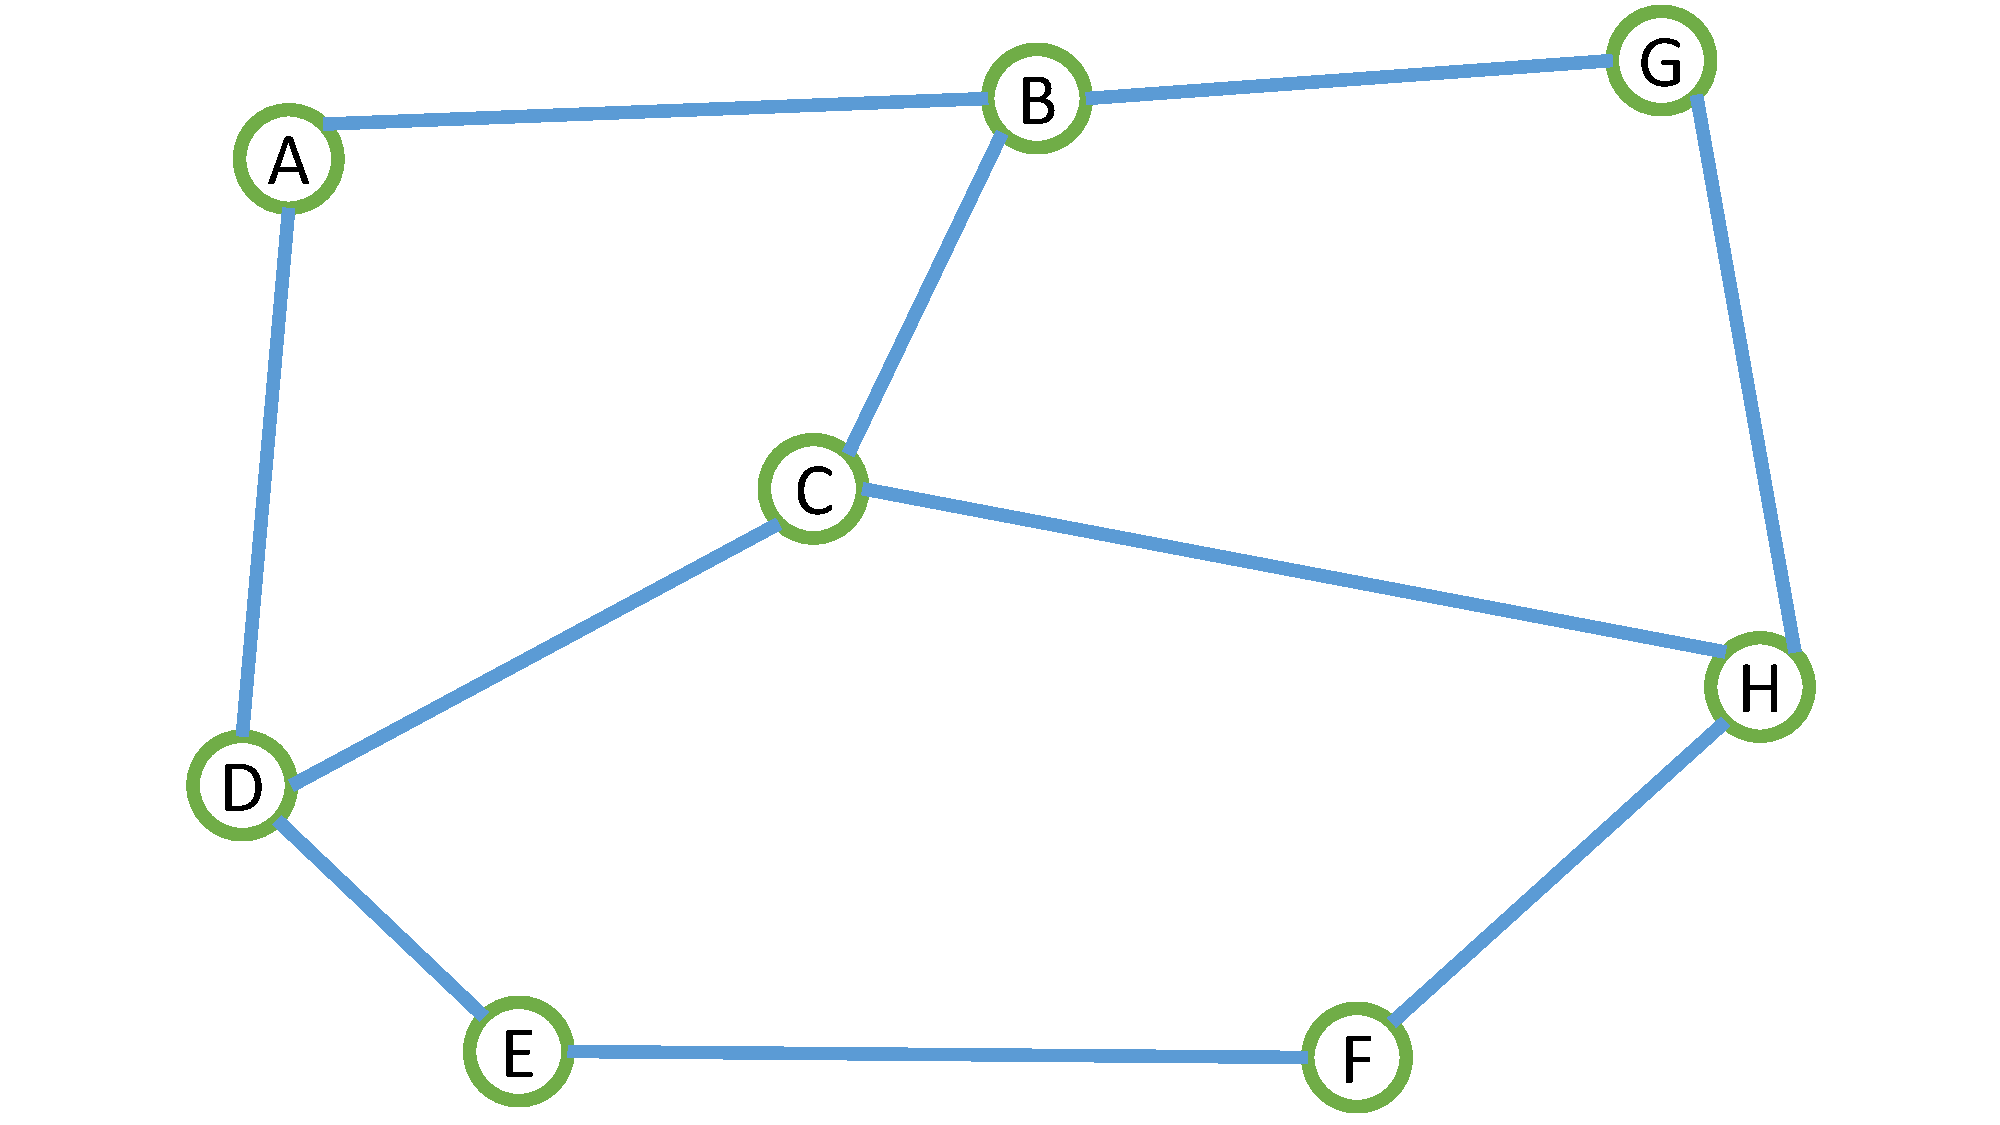
\includegraphics[scale=0.3]{Q4.pdf}
\end{figure}

الف) با استفاده از الگوریتم دایکسترا، کوتاهترین مسیر بین نودهای A و H را به دست آورید. تمام لینک‌ها، دارای وزن 1 هستند.

ب) فرض کنید مسیرهای نوری زیر در شبکه داده شده اند:
\begin{table}[h]
\centering
\begin{tabular}{|c|c|}
\hline
شماره‌ی مسیر نوری
&
مسیر
\\\hline
1
&
A-B-G-H
\\\hline
2
&
A-B-C
\\\hline
3
&
A-D-C-H
\\\hline
4
&
B-C-D
\\\hline
5
&
H-F-E-D
\\\hline
6
&
C-H-G-B
\\\hline
\end{tabular}
\end{table}

 روش های ابتکاری First-fit و Most-used را به اختصار توضیح دهید و با استفاده از آنها، به این مسیرهای نوری طول موج اختصاص دهید (لینک‌ها دو طرفه اند و هر لینک در هر جهت، دارای فیبر مجزا است).

\end{document}